\documentclass[12pt,a4paper,fleqn]{article}
\usepackage{rmpackages}																% usual packages
\usepackage{rmtemplate}																% graphic charter
\usepackage{rmexocptce}																% for DS with cptce eval

\usepackage{lipsum}

%\cfoot{} 													% if no page number is needed
%\renewcommand\arraystretch{1.5}		% stretch table line height

\begin{document}

\newcounter{int}
\setcounter{int}{1}
\loop

\begin{doc}
\textbf{Spectre d'émission de quelques espèces}

Le spectre d'émission d'un élément lui est caractéristique : voici ceux de quelques espèces.
\begin{center}
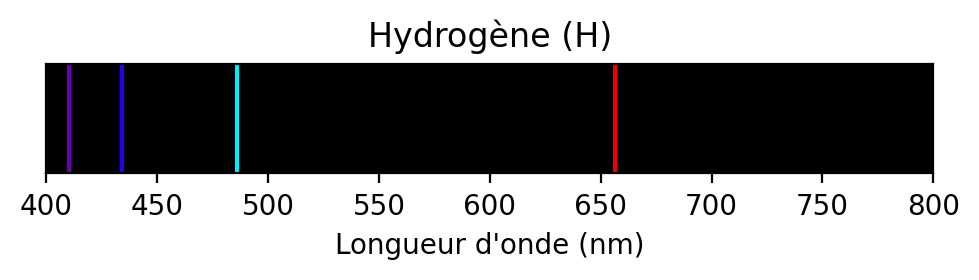
\includegraphics[width=.49\linewidth]{images/spectrum_H.png}
\hfill
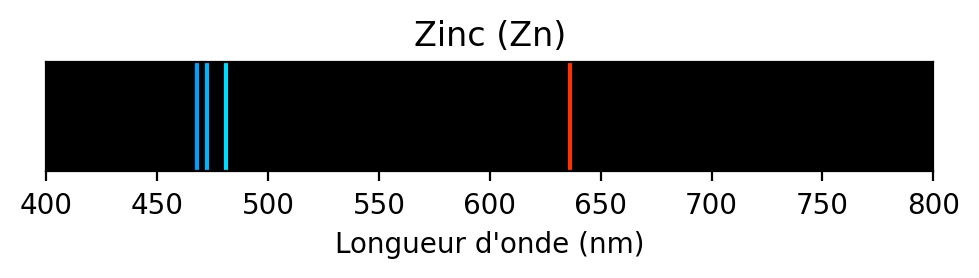
\includegraphics[width=.49\linewidth]{images/spectrum_Zn.png}

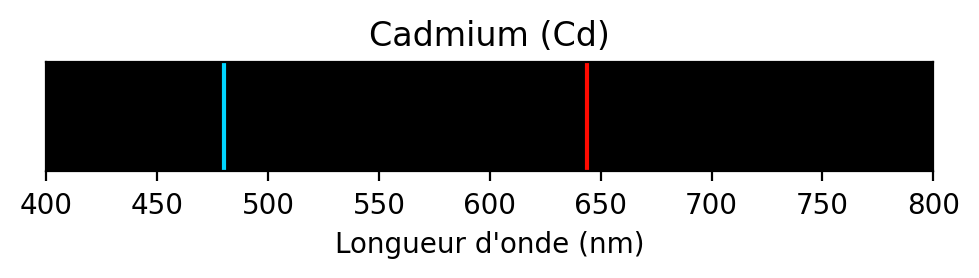
\includegraphics[width=.49\linewidth]{images/spectrum_Cd.png}
\hfill
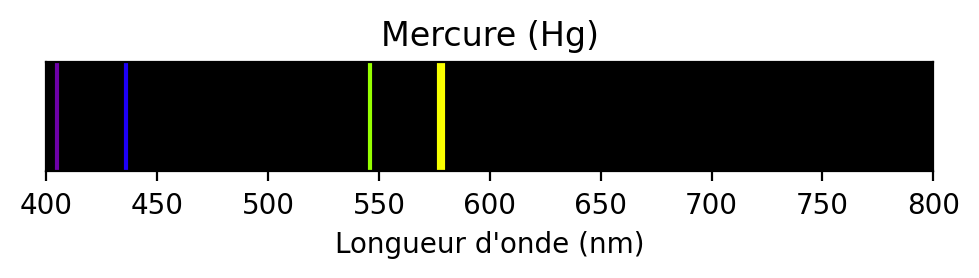
\includegraphics[width=.49\linewidth]{images/spectrum_Hg.png}
\end{center}
\end{doc}

\addtocounter{int}{1}
\ifnum \value{int}<4
\repeat

\end{document}

\begin{doc}
\textbf{Spectres d'émission de quelques espèces}

Le spectre d'émission d'un élément lui est caractéristique : voici ceux de quelques espèces.
\begin{center}
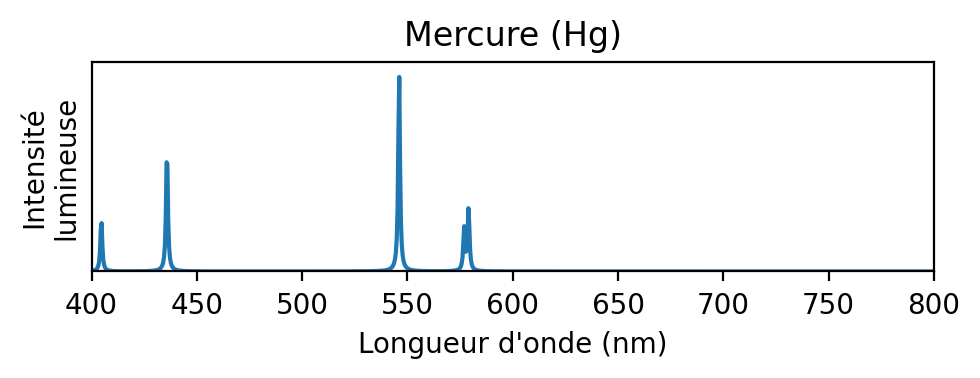
\includegraphics[width=.49\linewidth]{images/spectrum_curve_Hg.png}
\hfill
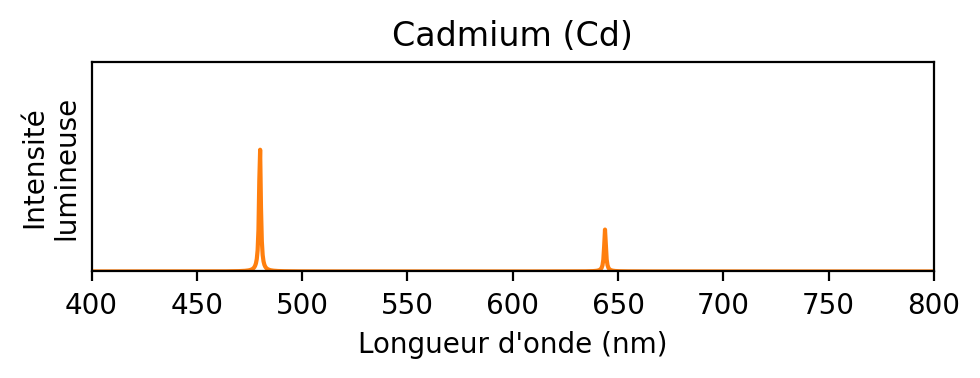
\includegraphics[width=.49\linewidth]{images/spectrum_curve_Cd.png}

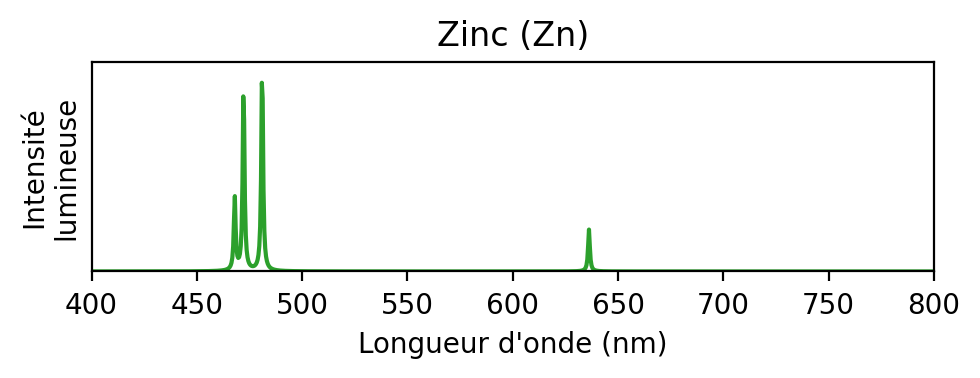
\includegraphics[width=.49\linewidth]{images/spectrum_curve_Zn.png}
\hfill
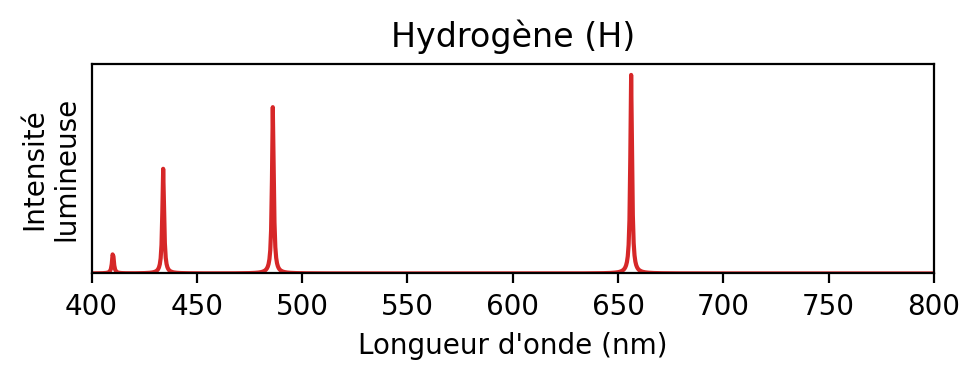
\includegraphics[width=.49\linewidth]{images/spectrum_curve_H.png}
\end{center}
\end{doc}

% Demander si certains ont des problème avec les couleurs

% Contextualisation

% Pendant 15 min, observer le spectre des lumières provenant des sources qui vous entourent. Comment pourrait-on les classer ?